\documentclass[letterpaper]{article}
\usepackage{graphicx}

\begin{document}

\title{A gossip-based protocol for exchanging immutable data in dynamic distributed environments}
\author{Adam Drescher \and Magdalena Cassel}
\date{}

\maketitle

\begin{abstract}
The abstract abstract.
\end{abstract}


\section{Introduction}
The proliferation of embedded networking is transforming homes into distributed computing environments.
A variety of devices, including desktops, laptops, tablets, printers, digital picture frames, televisions, digital cameras, and optical disc players, are now equipped with wireless network interfaces.
The ability of these devices to communicate with one another is creating opportunities for applications that engage multiple devices.
Typically, these networks will consist of a small to moderate number of devices, many of which are resource-constrained.
Home networks are built up as users contribute new devices to the network.
When a new device is added, i.e., turned on, the user expects the device to be available in a timely fashion.

Applications in home networks, and other dynamic distributed systems, are often governed by immutable configuration records contributed by each node in the system.
A simple directory application might gather and display a list of all of the devices in the system.
Similarly, applications using discovery and advertisement are governed by the service specifications and descriptions contributed by service consumers and providers.
One of the tasks in the system, then, is to match specifications to descriptions for the purpose of service binding.

Both centralized and distributed algorithms have been proposed to collect and process configuration records.
Centralized algorithms elect a leader which then facilitates query processing.
The leader may perform the processing itself or delegate processing to a subordinate node.
Distributed algorithms for configuration record processing often use one of two techniques, depending on the size of the records.
If the records are bigger than the maximum size of a message, i.e., a UDP packet, nodes discover other nodes using broadcast messages and then use point-to-point connections to collect remote configuration records.
Using this approach, the $n$th node to join the network will be queried $n-1$ times.
If the records are smaller than the maximum size of a message, nodes exchange configuration records using a multicast network, e.g., the Multicast Domain Name System.

To collect and process configuration records in home networks, we require a protocol that is both fully distributed and supports records of arbitrary size.
The resource-poor nature of the devices in the network, combined with the dynamic nature of the network, implies that a fully distributed algorithm is more appropriate.
In order to do capabilities-based matching, we require the ability to support configuration records of arbitrary size.
Finally, we would like to use gossip to avoid sending duplicate records when a new node joins the network.

This paper describes the Multicast File Transfer Protocol (MFTP), a distributed dissemination protocol for home networks that supports records of arbitrary size.

%Moving data across a network can take a variety of forms. 
%These forms correspond to different user needs and consequently different protocols. 
%Multicast File Transfer Protocol (MFTP) addresses the need to move immutable data between many different nodes in a fully distributed network. 
%% This is useful for 1) device discovery 2) File transfer in the absence of many technologies (including internet). the only thing that is necessary is computers with routing and broadcast/multicast enabled 3) maximizing the reach of a gossip style network

\section{Model\label{model}}

The two main tasks in configuration record processing are acquiring records from the network and establishing a relationship between two records.
We adopt the view that configuration records can be serialized and stored in a file.
The task of acquiring a record is then equivalent to downloading a file from the network.
Once a configuration record has been downloaded, its content can then be compared to configuration records that are stored locally.

A \emph{file} in MFTP is a finite sequence of bytes with an associated type.
Each file is uniquely identified by its \emph{file ID} which contains the file's type, length, and a hash of the file's contents.
The type is defined by the user and is used to limit the potential relationships among files.
We assume the existence of a user-defined predicate $\gamma(fid_1, fid_2)$ that returns true if there is potentially a relationship between the two files.
The predicate $\gamma$ is symmetric, i.e., $\gamma(fid_1, fid_2) = \gamma(fid_2, fid_1)$ and non-reflexive, i.e., $\gamma(fid_1, fid_1)$ is false.
Note that $\gamma$ is only defined using file IDs and can therefore only check file types and lengths.
We also assume the existence of a user-defined predicate $\mu(file_1, file_2)$ that returns true if a relationship between $file_1$ and $file_2$ exists.
Like $\gamma$, the predicate $\mu$ is symmetric and non-reflexive.
The predicate $\mu$ implies $\gamma$, i.e., $\mu(file_1, file_2) \to \gamma(fid(file_1), fid(file_2))$.

MFTP assumes that all communication takes place by sending fixed-size messages over a broadcast or multicast channel.
This allows MFTP to take advantage of gossip since file contents and matching relationships can be communicated efficiently to multiple interested parties.
To enable the sending of file contents using fixed-size messaging, we divide a file into pieces of equal size called \emph{fragments}.

The MFTP protocol contains three types of messages: fragments, requests, and matches.
Each message in MFTP is prefixed with a header indicating its type.
A \emph{fragment message} consists of a file ID, a fragment index, and the data comprising the indicated fragment.
A \emph{request message} consists of a file ID and a set of fragment indices.
For example, our implementation uses a set of spans where each span requests a contiguous set of fragments.
However, one can envision the request to contain more advanced structures, e.g., functions, that can define arbitrary sets.
A \emph{match message} consist of a file ID and a set of matching file IDs for which $\gamma$ is true.

Two files with the same content and type will have the same file ID.
With a strong enough hashing mechanism, we can assume two files are equal if their file IDs are the same.
Since the identity of a file is completely determined by its content, files are immutable and can be freely replicated.
Peers in the protocol are free to cache any fragment and respond to any requests for which they have a fragment.
The process of acquiring a file consists of repeatedly sending requests and receiving fragments from any peers that chose to respond until all of the fragments have been acquired.

Learning relationships can be accomplished in one of two ways.
First, peers in MFTP periodically send a fragment to announce the presence of the file in the network.
Assume that a peer serving $file_1$ receives an announcement for $file_2$.
The peer checks $\gamma(fid(file_1), fid(file_2))$ to determine whether a relationship is possible.
If a relationship is possible, the peer acquires the file and checks $\mu(file_1, file_2)$ to determine whether the relationship exists.
Peers periodically send match messages to indicate which files have a relationship with the file they serve.
The second way relationships can be learned is by eavesdropping on the match messages sent by other peers.

%%TODO: Talk about validation - possible coinage 'incremental digest'

\paragraph{Matching.}
Each MFTP automaton contains a flag that determines whether it will perform matching. 
It has another flag that determines whether it will self-destruct when it has finished downloading its file.
If the matching flag is set, the automaton applies the matching function $\iota$ to the file IDs of incoming fragments.
If $\iota$ is true, the automaton recursively constructs another MFTP automaton to download the potential match.
This child automaton does not perform matching.  
Its self-destruct flag is set so that it will self-destruct once the potential match has been downloaded.
When the download is complete, the parent automaton applies the matching function $\mu$ to the file to determine whether it is a match.

\section{Design}
%% General stuff -- The short argument is we're developing a new protocol
%% the I/O Automata formal model is good for modeling protocols, therefore we modeled it as an mftp automaton
%% Diagram with the 3 pieces
%% Describe the diagram, this is how we're going to do it, this is how we're interfaced and kinda put things together
%% then go into MFTP Automaton, state, etc
%% then go on and talk about the actions (send receive etc)

The I/O Automata formal model is a well-established technique for building protocols.
%% Talk about why I/O Automata is a good method (even though we didn't have a choice)
I/O Automata model stateful distributed system components that can interact and be composed with each other.
They change state through transitions classified as input, output or internal actions.
Input and output actions in different automata are bound; output actions in the one trigger input actions in the other.
As a result, we present our design of the MFTP protocol as automata.

\begin{figure}
  \center
  
\includegraphics[scale=0.65]{diagramOne}
  \caption{Basic implementational view of the protocol \label{DesignOne}}
\end{figure}

\ref{DesignOne} outlines the necessary pieces which constitute our protocol.
We define a basic MFTP automaton and a broadcast/multicast channel automaton.
We define a basic MFTP automaton, a sender, and a receiver.
The responsibilities of the MFTP automaton are to acquire data and to help others acquire it.

Each MFTP automaton begins with a file, encapsulated in a File object, which is either incomplete or complete.
If the file is incomplete, the automaton generates requests for the missing fragments.
If the file is complete, the automaton may serve the file, or it may serve the file while performing matching on it.

MFTP automata receive messages via the receive input action.
If the input message is a valid fragment of its own file, the automaton saves the fragment.
If the input message is a request for fragments of its file, it flags those fragments as having been requested.
If the input message is a match containing its file ID, it records the matching IDs for download.

The automaton holds a queue of one message to send. 
The internal actions which fill this queue are triggered periodically.
The automaton generates messages containing one requested fragment if any fragments in the file have been requested.
The fragment sent is selected at random to help avoid collisions with other MFTP automata serving the same file.
The automaton generates requests if some fragments in the automaton's own file are missing.
The automaton generates match messages if it has recorded any matches to its file.

The broadcast/multicast channel automaton uses the UDP sender and receiver built into ioa.
The channel may be connected to more than one MFTP automaton.

The automaton reports that its file is complete using the download complete output action.
%%  to multicast messages one at a time.
%%The receiving automaton uses the ioa UDP receiver.

\section{Implementation}
%% We implimented our IO Automata design using ioa framework
%% Interesting techniques - suicide, recursive automata

\section{Evaluation and Discussion\label{evaluation}}
\paragraph{Jam.} %%needs different header
Our implementation defines three file types, \emph{data}, \emph{meta} and \emph{query}.  
A data file contains data from any file in the network.
A meta file contains as data the file ID of a file in the network and its name. 
A query file contains only the name of the file which is being queried.

We wrote two programs, \emph{Share} and \emph{Get}, which use MFTP, sender and receiver automata to disseminate a file or files. %%Can one 'disseminate' a file?
Share creates two MFTP automata, \emph{file server} and \emph{meta server}.
File server is constructed with a complete file \emph{f}, and meta server is constructed with a meta file.
The meta file is generated from the fileID and name of f.
At the start, Get creates one MFTP automaton, \emph{query server}, constructed with a query file.
The query file is generated from the name of the file to download, supplied by a command line argument.

We defined a functor interface so that Share and Get could use different $\iota$ and $\mu$ functions.
In Share, meta server performs matching on the meta file and broadcasts matches to f.
Its $\iota$ returns true if the incoming file is a query file.
Its $\mu$ returns true if the contents of the downloaded query file match the name of f.

\begin{figure}
  \center
  
\includegraphics[scale=0.65]{share_diagram}
  \caption{The share program \label{EvaluationOne}}
\end{figure}

In Get, query server performs matching on the query file.
Its $\iota$ returns true if the incoming file is a meta file.
Its $\mu$ returns true if the contents of the downloaded meta file match the name of the file being queried.
Query server passes the meta files downloaded by its child automata to Get.
Using the file IDs contained in the meta files, Get constructs further MFTP automata which download the files pertaining to those file IDs.

\begin{figure}
  \center
  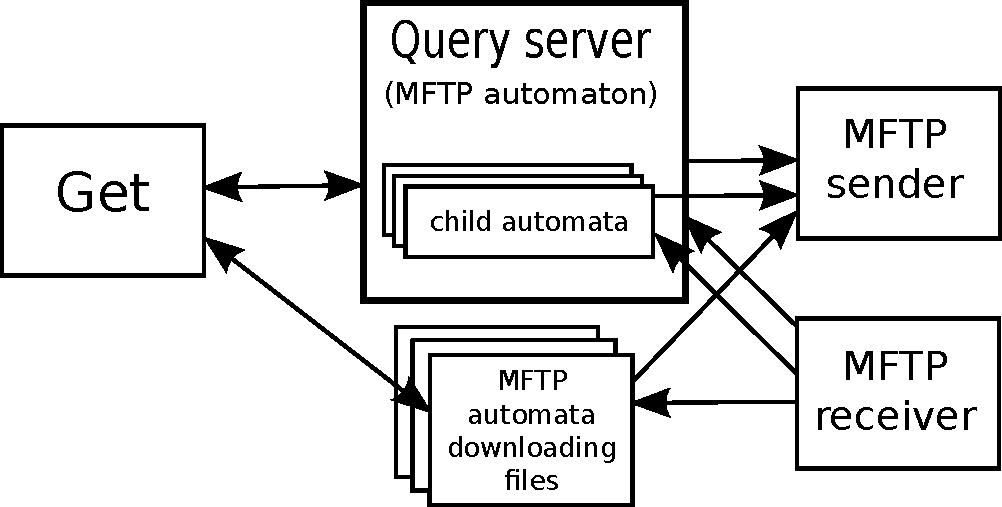
\includegraphics[scale=0.65]{get_diagram}
  \caption{The get program \label{EvalutationTwo}}
\end{figure}

\section{Adam's Section}
%% Go into more detail / provide more examples
A couple of things were hard to digest, the first of which being indirect triggers.  
It's hard to swallow the idea that you can queue an action but it's time of execution is far from guaranteed.  
The second hardest thing was simply the intimidation factor of realizing your entire summer would be working with an unknown, rather large library that nobody but the creator had used before--which was modelled after a complicated formalism I had never heard of that no one had bothered to fully develop since its inception.  
That's quite the pill to swallow.

One thing that I learned was easy was to model the automata very closely to Lynch's design.  
It was much easier for me to learn the relationship between the formalism and the code by looking at well-modelled automata, so the same would extend onto someone looking at the formalism and our code. 
Maintaining this allows for a less steep learning curve, and hopefully contributes to the automata maintaining their structural integrity as more people use the library.
An example of this would be correctly classifying input, output, and internal actions.

It's hard to describe what is ``harder'' to implement using I/O Automata.  
Though I/O Automata present a \emph{different} problem set than using threads, the resulting problem set is respectively easier and more intuitive to handle.  

However, what is easer to implement is much more plentiful.
The design and debugging of the program is much more intuitive.
It allowed for a high degree of abstraction, which is key for easily-understandable code.
It allowed \emph{extremely} easy refactoring of any class when compared to the alleged dregs of refactoring a thread-intensive class.

In regards to building a protocol, I learned that it is extremely helpful to add and then test small bits of functionality at a time, in order to get a small working product.
Once this is complete, repeat by adding or extending the functionality.
Though this may seem trivial, calculated baby-steps made developing a protocol seem much easier than trying it all at once.
For example, developing a simple transfer channel to correctly model our mftp automaton.  After this was well tested, we then moved it to transfer over multicast/broadcast.

\section{Magnum Albatross}
The most challenging part of learning to work with I/O Automata was to think of the \"events\" in the system not as interrupts that immediately trigger an action, but rather as transitions that change the state of the automaton to enable and disable other actions.

\section{Related Work}

\section{Conclusion}

\end{document}


%% \paragraph {Files.}
%% The main concept in MFTP is that of a \emph{file}.
%% A file is a sequence of bytes with a length and a user-defined type.
%% Files are divided into pieces of equal size called \emph{fragments}.
%% Each file is uniquely identified by a \emph{file ID} that contains the file's type, length, and a hash of the file's contents.

%% \paragraph{Messages.}
%% File transfer takes place via \emph{messages}.
%% There are three types of messages in the protocol.
%% The first message type is a \emph{request}.
%% A request contains a file ID and a set of fragment indices.
%% We implemented requests as the file ID and a set of contiguous regions.  
%% However, one can envision the request to contain anything that defines a set.
%% The second message type is a \emph{fragment}, which consists of a file ID, a fragment index, and the data comprising that fragment of the file.
%% Last is a \emph{match}, which consists of a file ID and a set of matching file IDs.

%% \paragraph {Tasks.}
%% The two main tasks in MFTP are acquiring a file and establishing a relationship between two files.
%% The process of acquiring a file involves sending a request for the file's fragments and receiving fragments sent in response.
%% MFTP is a peer-to-peer protocol because each participant can act as both a client and a server.
%% A peer can send out any fragments for which it gets a request.
%% Fragments are periodically broadcast, even in the absence of requests, to indicate what files exist in the network.
%% A peer can use requests to poll for fragments of a file which can span from individual fragments to the whole file.
%% A peer which has successfully downloaded any number of fragments of a file can then serve those fragments.

%% Matching is a two-step process.
%% The first step applies a matching function $\iota$ to two file IDs to determine whether a match is possible between the two files.  
%% The second step applies a matching function $\mu$ to the two files to determine whether there is a match.
%% If $\mu$($f_1$,$f_2$) is true, $\iota$($fid_1$,$fid_2$) must be true.
%% However, if $\iota$($fid_1$,$fid_2$) is true, $\mu$($f_1$,$f_2$) does \emph{not} have to be true. 

%% The problem of processing configuration information can be cast using relational database techniques.
%% A database consists of one or more tables, where each table consists of a number of identically structured records.
%% Database tables are manipulated by the insert, delete and update methods, which insert, delete and modify records.
%% Database tables are queried using the select operator.
%% For processing configuration information, each configuration record is mapped into a table of the appropriate type.
%% Listing all of the components in the system corresponds to selecting all of the records in the database.
%% Discovery can be accomplished by projecting a service specification record onto the table of service descriptions.

%% A record is defined by its content.
%% Consequently, each record is immutable and the update method is not allowed.
%% Configuration records are immutable and under the control of the node that stores them.

%% Each record is immutable. Update doesn't exist. The records stored on each node are under the control of that node. Insert and delete only exist locally.

%% Each table and each record has an ID
%% Each record ID consists of the ID of the table it belongs to and the length and hash of its binary representation.
%% The records are uniquely identifiable by their IDs.
%% Each node then contributes zero or more immutable records to one or more of the tables.
%% We can consider each configuration item as a record in a read-only database.

%% Each record is locally controlled
%% since immutable, can be replicated (no duplicates in the database)
%% each node has its own set of records which it contributes
